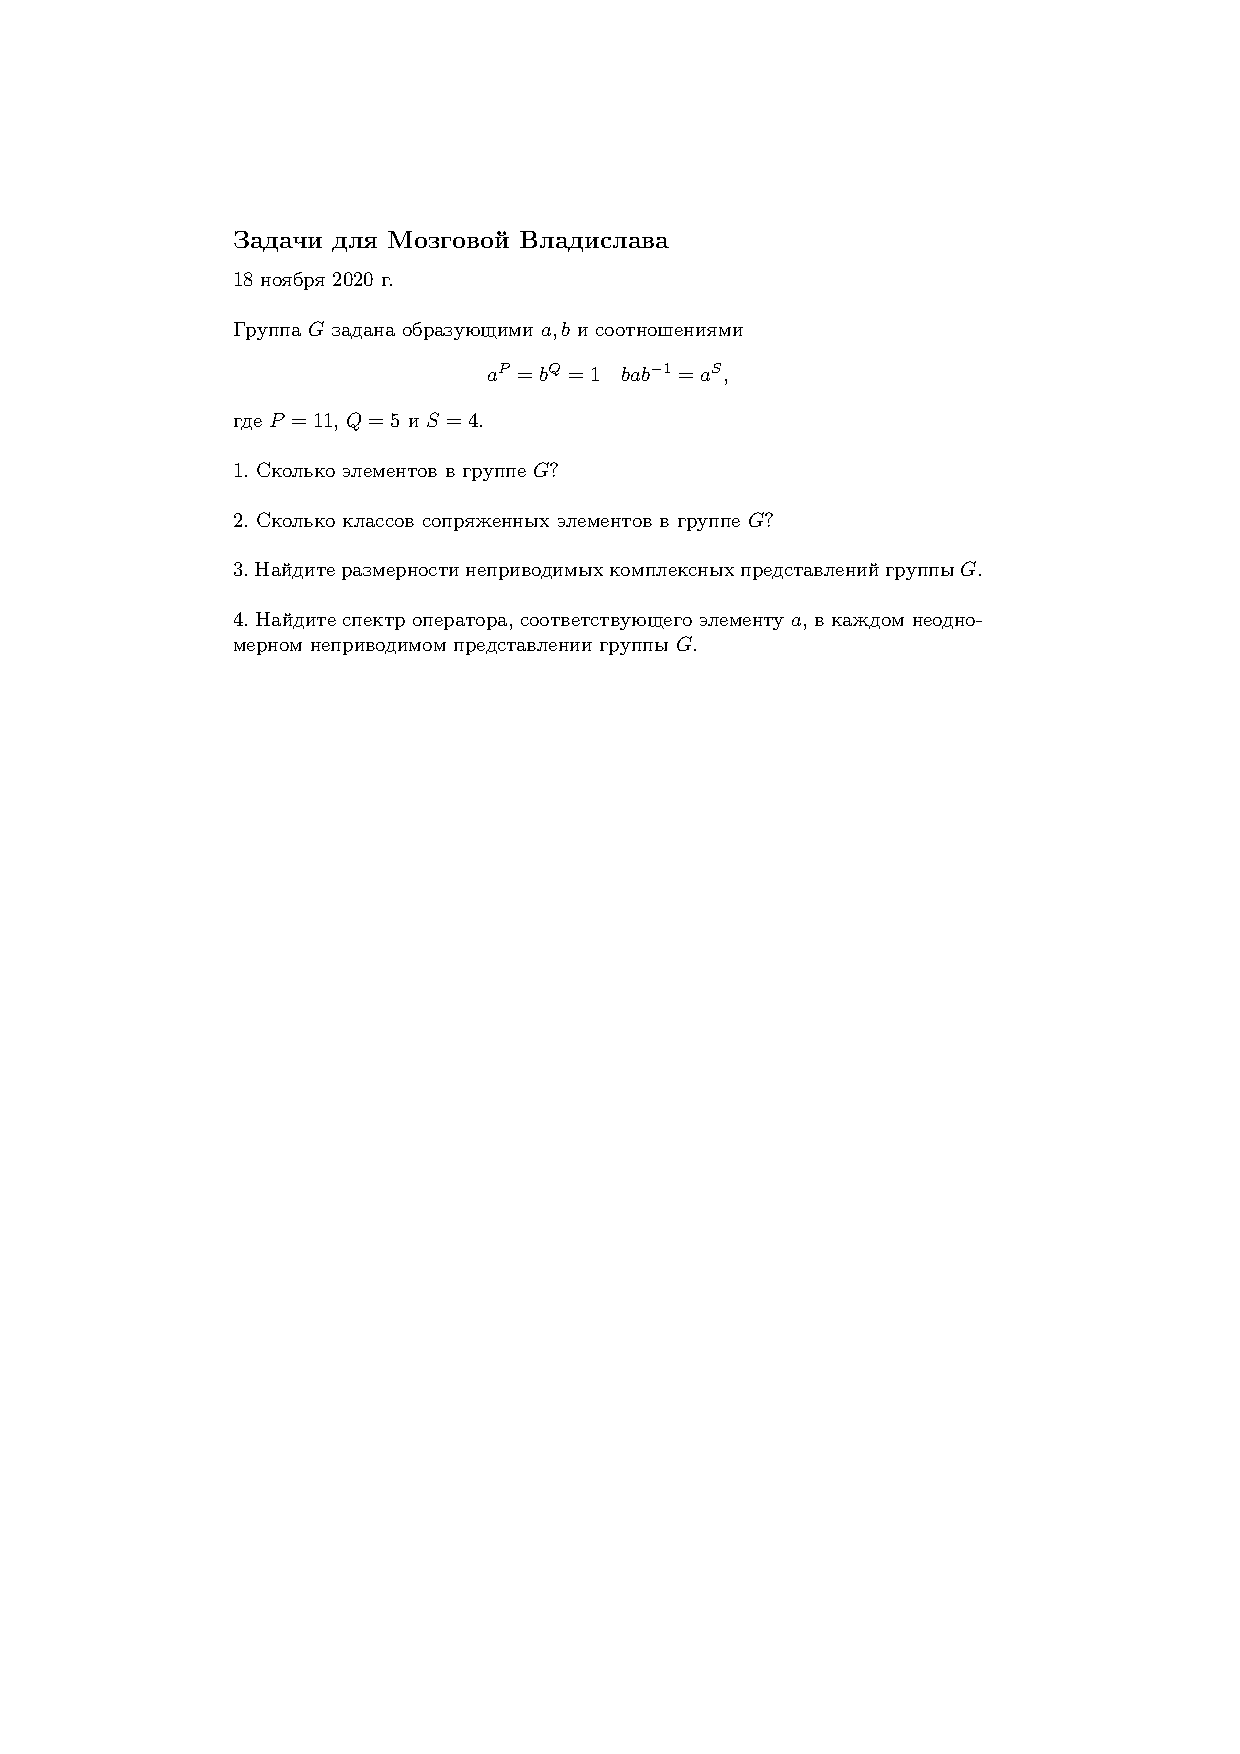
\includepdf[scale=0.95,pages=1,pagecommand=\section*{Условия}]{Tasks/problem2}
\newpage
\section*{Решения}
\subsection*{Задача 1}
	Так как $a,b$ -- образующие группы $G$, то $G = \{a^{m}b^{n}|\ m \in \{0, \ldots, 10\},\ n \in \{0,\ldots,4\}\}$.\\
	Заметим, что любой элемент представим в виде $a^{i}b^{j}$ так как в последовательности из $a$ и $b$ мы можем заменять $ba$ на $a^4 b$, при этом не существует $i,j,k,l:\ a^{i}b^{j} = a^{k}b^{l}$, так как $a^{i}b^{j} = a^{k}b^{l}\ \Leftrightarrow\ a^{i-k}b^{j-l} = 1$, но тогда мы знаем, что $(i-k) \divby 11,\ (j-l) \divby 5$, а следовательно $i \equiv k \mod 11,\ j \equiv l \mod 5$.\\
	Тогда $G = \{a^{m}b^{n}|\ m \in \{0, \ldots, 10\},\ n \in \{0,\ldots,4\}\}$, а следовательно $|G| = 5 \cdot 11 = 55$
	
\subsection*{Задача 2}
	(количество элементов класс сопряженности)|(порядок группы), следовательно количество элементов классов сопряженности может быть только $1,5,11,55$, но $55$ быть не может, так как $h 1 h^{-1} = 1$, следовательно $\{1\}$ -- класс сопряженности состоящий из одного элемента.\\
	Класс сопряженности $\{hgh^{-1}| g \text{ фиксированное }, h \in G\}$\\
	Рассмотрим $g$ -- элемент $N_{11} = a^k$
	\begin{gather*}
		b a^{k} b^{-1} = a^4 b a^{k-1} b^{-1} = a^{4k}\\
		a^{k} \to a^{4k} \to a^{5k} \to a^{9k} \to a^{3k}\\
		N_{11} = \{1\} \cup \{a, a^4, a^5, a^9, a^3\} \cup \{a^2, a^8, a^{10}, a^7, a^6\}
	\end{gather*}
	Рассмотрим как выглядит орбита $b$
	\begin{gather*}
		(a^x b^y) b (a^x b^y) = a^x b^y b b^{-y} a^{-x} = a^x b a^{-x}
	\end{gather*}
	То есть элемент вида $a^i b$\\
	Покажем, что любой такой мы можем получить:
	\begin{gather*}
		a^{-x} b a^{x} = a^{-x} a^{4} b a^{x-1} = a^{-x} a^{4} \ldots a^{4} b = a^{4x} b
	\end{gather*}
	Заметим, что $\operatorname{gcd}(4,11) = 1$, следовательно с помощью $3x$ можно получить все остатки по $\mod 11$, заметим, что в данном класс сопряженности ровно 31 элемент.\\
	Класс элемента $b^2$\\
	Заметим, что в классе сопряженности есть элементы только вида $a^i b^2$:
	\begin{gather*}
		(a^x b^y) b^2 (a^x b^y)^{-1} = a^x b^y b^2 b^{-y} a^{-x} = a^x b^2 a^{-x} = a^{x} a^{-x \cdot 4^2} b^2 = a^{i} b^2
	\end{gather*}
	Тогда
	\begin{gather*}
		a^{-x} b^2 a^{x} = a^{-x} a^{4^2 x} b^2 = a^{5x} b
	\end{gather*}
	Заметим, что $\operatorname{gcd}(5,11) = 1$, а следовательно таким образом можно получить любой остаток по $\mod 31$, следовательно все элементы вида $a^i b^2$ лежат в одном классе сопряженности.\\
	Также для $a^i b^3$
	\begin{gather*}
		(a^x b^y) b^3 (a^x b^y)^{-1} = a^x b^y b^3 b^{-y} a^{-x} = a^x b^3 a^{-x} = a^{x} a^{-x \cdot 4^3} b^3 = a^{i} b^3\\
		a^{-x} b^3 a^{x} = a^{-x} a^{4^3 x} b^3 = a^{9x} b^3\\
		\operatorname{gcd}(9,11)=1
	\end{gather*}
	И для $a^i b^4$
	\begin{gather*}
		(a^x b^y) b^4 (a^x b^y)^{-1} = a^x b^y b^4 b^{-y} a^{-x} = a^x b^4 a^{-x} = a^{x} a^{-x \cdot 4^4} b^4 = a^{i} b^4\\
		a^{-x} b^4 a^{x} = a^{-x} a^{4^4 x} b^4 = a^{3x} b^4\\
		\operatorname{gcd}(3,11)=1
	\end{gather*}
	Следовательно всего классов сопряженности $3 + 4 = 7$
	
	
\newpage
\subsection*{Задача 3}
	Известно, что существует 7 классов сопряженных элементов, а следовательно 7 неприводимых представлений. $x_i = \dim \rho_i$, причем $\sum x_i^1 = |G| = 55$\\
	Рассмотрим одномерные представления. $a,b$ -- образующая
	\begin{gather*}
		\rho(a) = x\quad a^{11} = 1,\ x^{11} = 1,\ x \in \mathbb{C}\\
		\rho(b) = y\quad a^{5} = 1,\ y^{5} = 1,\ y \in \mathbb{C}\\
		\rho(b) \rho(a) \rho(b^{-1}) = yxy^{-1} = x^{4}\\
		x = x^{4} \Leftrightarrow 1 = x^{3}
	\end{gather*}
	Но $x^{11} = 1$, а следовательно $x=1$ (так как $\operatorname{gcd}(11,3) = 1$)\\
	$b^5 = 1\ \Rightarrow b = 1, \omega, \omega^{2}, \omega^{3}, \omega^{4}$\\
	Следовательно существует 5 одномерных представлений.\\
	Посмотрим, существуют ли двумерные представления\\
	Пусть $\rho$ -- неприводимое двумерное
	\begin{gather*}
		\rho(a) = A \in GL_2(\mathbb{C})\quad A^{11} = E\\
		\rho(b) = B \in GL_2(\mathbb{C})\quad B^{5} = E
	\end{gather*}
	Заметим, что так как $A^{11} = E$, то она диагонализуема и
	\begin{gather*}
		A = 
		\begin{pmatrix}
			x & 0 \\ 0 & y
		\end{pmatrix}
		\in GL_2(\mathbb{C})\\
		B = 
		\begin{pmatrix}
			k & l \\ m & n
		\end{pmatrix}
		\text{ -- в том же базисе}\\
		BA = A^{4}B\\
		\begin{pmatrix}
			kx & ly \\ mx & ny
		\end{pmatrix}
		=
		\begin{pmatrix}
			k & l \\ m & n
		\end{pmatrix}
		\begin{pmatrix}
			x & 0 \\ 0 & y
		\end{pmatrix}
		=
		\begin{pmatrix}
			x^{4} & 0 \\ 0 & y^{4}
		\end{pmatrix}
		\begin{pmatrix}
			k & l \\ m & n
		\end{pmatrix}
		=
		\begin{pmatrix}
			x^{4} k & x^{4} l \\ y^{4} m & y^{4} n
		\end{pmatrix}
	\end{gather*}
	Получим систему
	\begin{gather*}
	\begin{cases}
		kx = x^{4} k\\
		ly = x^{4} l\\
		mx = y^{4} m\\
		yn = n y^{4}
	\end{cases}\\
	k,n = 0\qquad m,l \ne 0\\
	\begin{pmatrix}
		k & l \\ m & n
	\end{pmatrix}
	=
	\begin{pmatrix}
		0 & l \\ m & 0
	\end{pmatrix}
	\text{ -- невырождена}\\
	\begin{cases}
		ly = x^{4}l\\
		mx = y^{4}m
	\end{cases}\qquad
	\begin{cases}
		y = x^{4}\\
		x = y^{4}
	\end{cases}\\
	y = x^{4} = y^{4^{4}} = y^{16} = y^{5}\quad y = 1\\
	A =
	\begin{pmatrix}
		1 & 0 \\ 0 & 1
	\end{pmatrix}
	\end{gather*}
	Противоречие с неприводимостью, так как у $B$ существует хотя бы один собственные вектор, а следовательно и для $A = E$ он тоже будет собственным.\\
	Далее заметим, что $5^2 = 4^2 + 3^2$, то есть 3 и 4 мерных представлений либо 0, либо 2, так как иначе $55 \ne x_1^2 + x_2^2 + x_3^2 + x_4^2 + x_5^2 + x_6^2 + x_7^2$. Тогда доказав, что нет 2 представлений 3 или 4 степени, мы докажем, что все остальные представления имеют степень 1 или 5, то есть
	\begin{gather*}
		55 = x_1^2 + \ldots + x_7^{2} \text{ , где } x_1 = x_2 = x_3 = x_4 = x_5 = 1 \text{ и } x_i \geqslant 5 \text{ при } i \geqslant 6\\
		50 = x_6^2 + x_7^2 = 5^2 + 5^2
	\end{gather*}
	Равенство достигается и все остальные представления пятимерны.\\
	То есть существует 5 одномерных и 2 пятимерных представления
	
\newpage
\subsection*{Задача 4}
	Пусть $\rho$ -- пятимерное неприводимое представление
	\begin{gather*}
		\rho(a) = A \in GL(5,\mathbb{C})\quad A^{11} = E\\
		\rho(b) = B \in GL(5,\mathbb{C})\quad B^{5} = E\\
		A =
		\begin{pmatrix}
			a_1 & 0 & 0 & 0 & 0\\
			0 & a_2 & 0 & 0 & 0\\
			0 & 0 & a_3 & 0 & 0\\
			0 & 0 & 0 & a_4 & 0\\
			0 & 0 & 0 & 0 & a_5
		\end{pmatrix}\qquad
		A^4 = 
		\begin{pmatrix}
			a_1^4 & 0 & 0 & 0 & 0\\
			0 & a_2^4 & 0 & 0 & 0\\
			0 & 0 & a_3^4 & 0 & 0\\
			0 & 0 & 0 & a_4^4 & 0\\
			0 & 0 & 0 & 0 & a_5^4
		\end{pmatrix}\qquad
		BAB^{-1} = A^{4}
	\end{gather*}
	$A$ и $A^4$ сопряжены, а следовательно у них совпадают ЖНФ, следовательно ${a_1^4, a_2^4, a_3^4, a_4^4, a_5^4}$ -- перестановка $\{a_1,a_2,a_3,a_4,a_5\}$
	\begin{gather*}
		A^{11} = E\\
		a_1 = \sqrt[11]{1} = 1,\omega,\ldots,\omega^{10}\\
		\vdots\\
		a_5 = \sqrt[11]{1} = 1,\omega,\ldots,\omega^{10}
	\end{gather*}
	Перестановка не тождественна, так как иначе $a_1 = a_2 = a_3 = a_4 = a_5 = 1$ и представление приводимо\\
	Перестановка $(ij)$
	\begin{gather*}
		\begin{cases}
			a_1^4 = a_2\\
			a_2^4 = a_1\\
			a_3^4 = a_3\\
			a_4^4 = a_4\\
			a_5^4 = a_5
		\end{cases}\qquad
		\begin{cases}
			a_1 = a_2^4 = a_1^{16}\\
			a_1^{11} = a_2^{11}\\
			a_3^4 = a_3\\
			a_4^4 = a_4\\
			a_5^4 = a_5
		\end{cases}\qquad
		a_1 = a_2 = 1
		\text{ представление приводимо}
	\end{gather*}
	Перестановка $(ijk)$
	\begin{gather*}
		\begin{cases}
			a_1^4 = a_2\\
			a_2^4 = a_3\\
			a_3^4 = a_1\\
			a_4^4 = a_4\\
			a_5^4 = a_5
		\end{cases}\qquad
		\begin{cases}
			a_1 = a_2^4 = a_3^{4^2} = a_1^{4^3}\\
			a_1^{11} = a_2^{11} = a_3^{11}\\
			a_4^4 = a_4\\
			a_5^4 = a_5
		\end{cases}\qquad
		a_1 = a_2 = a_3 = 1
		\text{ представление приводимо}
	\end{gather*}
	Перестановка $(ijkl)$
	\begin{gather*}
		\begin{cases}
			a_1^4 = a_2\\
			a_2^4 = a_3\\
			a_3^4 = a_4\\
			a_4^4 = a_1\\
			a_5^4 = a_5
		\end{cases}\qquad
		\begin{cases}
			a_1 = a_2^4 = a_3^{4^2} = a_4^{4^3} = a_1^{4^4}\\
			a_1^{11} = a_2^{11} = a_3^{11} = a_4^{11}\\
			a_5^4 = a_5
		\end{cases}\qquad
		a_1 = a_2 = a_3 = a_4 = 1
		\text{ представление приводимо}
	\end{gather*}	
	Перестановка $(ijklm)$
	\begin{gather*}
		\begin{cases}
			a_1^4 = a_2\\
			a_2^4 = a_3\\
			a_3^4 = a_4\\
			a_4^4 = a_5\\
			a_5^4 = a_1
		\end{cases}\qquad
			a_1 = a_2^4 = a_3^{4^2} = a_4^{4^3} = a_5^{4^4}
	\end{gather*}
	Рассмотрим циклы $x \to x^4 \to x^{4^2} \to \ldots$
	\begin{gather*}
		a \to a^4 \to a^5 \to a^9 \to a^3 \to a\\
		a^2 \to a^8 \to a^{10} \to a^7 \to a^6 \to a
	\end{gather*}
	Существует 2 цикла длины 5, 0 циклов длины 4,3,2 и 1 цикл длины 1\\
	Ответ:\\
	1) $(a, a^4, a^5, a^9, a^3)$\\
	2) $(a^2, a^8, a^{10}, a^7, a^6)$